% comment out for student version
\ifdefined\Student\relax\else\def\Teacher{}\fi

\documentclass[12pt]{article}

\title{Arrays of Arrays}
\author{Chris Mayfield, Helen Hu, and Dee Weikle}
\date{Summer 2021}

%\ProvidesPackage{cspogil}

% fonts
\usepackage[utf8]{inputenc}
\usepackage[T1]{fontenc}
\usepackage{mathpazo}

% spacing
\usepackage[margin=2cm]{geometry}
\renewcommand{\arraystretch}{1.4}
\setlength{\parindent}{0pt}

% orphans and widows
\clubpenalty=10000
\widowpenalty=10000
\pagestyle{empty}

% figures and tables
\usepackage{graphicx}
\usepackage{multicol}
\usepackage{tabularx}
\usepackage{wrapfig}

% fixed-width columns
\usepackage{array}
\newcolumntype{L}[1]{>{\raggedright\let\newline\\\arraybackslash\hspace{0pt}}m{#1}}
\newcolumntype{C}[1]{>{\centering\let\newline\\\arraybackslash\hspace{0pt}}m{#1}}
\newcolumntype{R}[1]{>{\raggedleft\let\newline\\\arraybackslash\hspace{0pt}}m{#1}}

% include paths
\makeatletter
\def\input@path{{Models/}{../../Models/}}
\graphicspath{{Models/}{../../Models/}}
\makeatother

% colors
\usepackage[svgnames,table]{xcolor}
\definecolor{bgcolor}{HTML}{FAFAFA}
\definecolor{comment}{HTML}{007C00}
\definecolor{keyword}{HTML}{0000FF}
\definecolor{strings}{HTML}{B20000}

% table headers
\newcommand{\tr}{\bf\cellcolor{Yellow!10}}

% syntax highlighting
\usepackage{textcomp}
\usepackage{listings}
\lstset{
    basicstyle=\ttfamily\color{black},
    backgroundcolor=\color{bgcolor},
    numberstyle=\scriptsize\color{comment},
    commentstyle=\color{comment},
    keywordstyle=\color{keyword},
    stringstyle=\color{strings},
    columns=fullflexible,
    keepspaces=true,
    showlines=true,
    showstringspaces=false,
    upquote=true
}

% code environments
\newcommand{\java}[1]{\lstinline[language=java]{#1}}%[
\lstnewenvironment{javalst}{\lstset{language=java,backgroundcolor=}}{}
\lstnewenvironment{javabox}{\lstset{language=java,frame=single,numbers=left}\quote}{\endquote}

% PDF properties
\usepackage[pdftex]{hyperref}
\urlstyle{same}
\makeatletter
\hypersetup{
  pdftitle={\@title},
  pdfauthor={\@author},
  pdfsubject={\@date},
  pdfkeywords={},
  bookmarksopen=false,
  colorlinks=true,
  citecolor=black,
  filecolor=black,
  linkcolor=black,
  urlcolor=blue
}
\makeatother

% titles
\makeatletter
\renewcommand{\maketitle}{\begin{center}\LARGE\@title\end{center}}
\makeatother

% boxes [optional height]
\newcommand{\emptybox}[1][10em]{
\vspace{1em}
\begin{tabularx}{\linewidth}{|X|}
\hline\\[#1]\hline
\end{tabularx}}

% models
\newcommand{\model}[1]{\section{#1}\nopagebreak}
\renewcommand{\thesection}{Model~\arabic{section}}

% questions
\newcommand{\quest}[1]{\subsection*{Questions~ (#1)}}
\newcounter{question}
\newcommand{\Q}{\vspace{1em}\refstepcounter{question}\arabic{question}.~ }
\renewcommand{\thequestion}{\#\arabic{question}}

% sub-question lists
\usepackage{enumitem}
\setenumerate[1]{label=\alph*)}
\setlist{itemsep=1em,after=\vspace{1ex}}

% inline answers
\definecolor{answers}{HTML}{C0C0C0}
\newcommand{\ans}[1]{%
\ifdefined\Student
    \leavevmode\phantom{~~\textcolor{answers}{#1}}
\else
    ~~\textcolor{answers}{#1}
\fi}

% longer answers [optional height]
\newsavebox{\ansbox}
\newenvironment{answer}[1][4em]{
\nopagebreak
\begin{lrbox}{\ansbox}
\begin{minipage}[t][#1]{\linewidth}
\color{answers}
}{
\end{minipage}
\end{lrbox}
\ifdefined\Student
    \phantom{\usebox{\ansbox}}%
\else
    \usebox{\ansbox}%
\fi}


\begin{document}

\maketitle

In Java, a multidimensional array is an array whose elements are themselves arrays.
You can declare an ``array of arrays'' by using two or more sets of brackets, such as \java{String[][]}.

\rolenames

\guide{
  \item Write nested for loops to traverse a two-dimensional array.
  \item Explain differences between rectangular and ragged arrays.
  \item Use two-dimensional arrays to model real-world problems.
}{
  \item Rewriting a group of repetitive statements as a for loop. (Information Processing)
}{
Make sure students have access to the source code.

Encourage the presenters and recorders to work together on the second half of \ref{model1.tex}.
For example, the presenter can direct message the final code to the recorder, or the recorder can simply retype everything the presenter does in real time.

Key questions: \ref{key1} and \ref{key2}
}

\model{Arrays}

An array variable stores a \emph{reference} to an array object.
We draw references as arrows, because they ``point'' to other memory locations.

\medskip
\begin{javalst}
    int[] data = null;


    int[] counts = {10, 3, 7, -5};


    double[] scores = new double[3];
\end{javalst}

\vspace{-9.75em}
\hfill 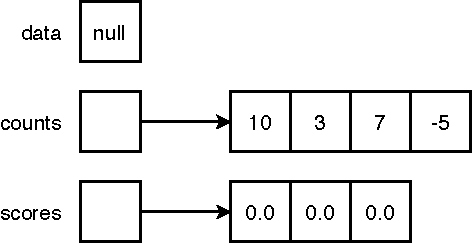
\includegraphics{diagram-array.pdf}
\hspace{2em} \null

\vspace{1.25em}
When passing an array to a method, only the reference is copied:

\medskip
\begin{javalst}
public static void printArray(int[] a) {
    System.out.print("{" + a[0]);
    for (int i = 1; i < a.length; i++) {
        System.out.print(", " + a[i]);
    }
    System.out.println("}");
}

public static void main(String[] args) {
    int[] nums = {159, 227};
    printArray(nums);
}
\end{javalst}

\vspace{-14em}
\hfill 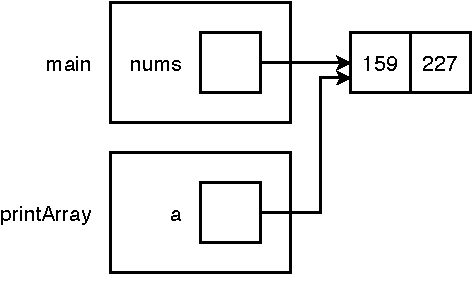
\includegraphics{diagram-array2.pdf}
\vspace{2em}


\quest{15 min}


\Q What is the length of each array?

\begin{multicols}{2}
\begin{enumerate}
\item \java{counts}? \ans[3em]{4}
\item \java{scores}? \ans[3em]{3}
\item \java{nums}?   \ans[3em]{2}
\item \java{a}?      \ans[3em]{2}
\end{enumerate}
\end{multicols}


\Q Looking at both diagrams above:

\begin{enumerate}
\item How many array variables were declared? \ans[3em]{5}
\item How many array objects were created? \ans[3em]{3}
\end{enumerate}


\Q Based on the top diagram, what is different about the variable named \java{data}?

\begin{answer}[3em]
The variable is \jans{null}, so there is no reference and no array object.
\end{answer}


\Q \label{key1}
Based on \java{counts} and \java{scores}, describe two ways that array objects can be created.
How are these two ways different from each other?

\begin{answer}[5em]
Arrays can be created either with curly braces or with the \jans{new} keyword.
The curly braces specify the initial values of array elements.
The \jans{new} keyword creates an array of specified length and initializes its elements to zero.
\end{answer}


\Q If the \java{printArray} method were to modify the array contents, would that change be visible in the \java{main} method?
Explain your reasoning.

\begin{answer}[3em]
Yes, because the variable \java{nums} and the variable \java{a} reference the same object.
\end{answer}


\Q Draw (or describe) a diagram of the following source code:

\begin{javalst}
int[] data = {1, 2, 3};
int[] copy = data;
\end{javalst}

\begin{answer}[15em]
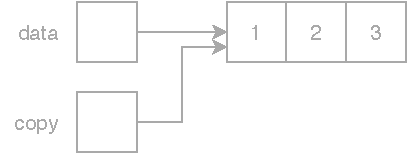
\includegraphics[scale=1]{data-copy.pdf}
\end{answer}


\Q (Optional) Paste the contents of \textit{Arrays.java} into \href{https://cscircles.cemc.uwaterloo.ca/java_visualize/#code=public+class+ClassNameHere+%7B%0A++++public+static+void+main(String%5B%5D+args)+%7B%0A++++++++%0A++++%7D%0A%7D&mode=edit&showStringsAsObjects=1}{Java Visualizer}.
What differences do you notice between the diagram in Java Visualizer and those in \ref{\currfilename}?

\begin{answer}
Answers might include:
\bull The variables are drawn in (method) frames.
\bull The array objects show the index of each cell.
\end{answer}

\clearpage
\model{Map of Team Names}

The following abbreviations are for National Football League (NFL) teams:

\begin{center}
\begin{tabular}{l|l}
ATL & Atlanta Falcons \\ \hline
DEN & Denver Broncos \\ \hline
IND & Indianapolis Colts \\ \hline
MIA & Miami Dolphins \\ \hline
SEA & Seattle Seahawks \\
\end{tabular}
\end{center}

Complete the table below using \textit{JShell} (the same way you did for \ref{model1.tex}).

\setlength{\defaultwidth}{20.8em}

\begin{center}
\begin{tabular}{|l|p{21em}|}
\hline
\multicolumn{1}{|c|}{\tr Java code} &
\multicolumn{1}{ c|}{\tr Shell output}
\\ \hline

\java{Map<String, String> teams;}
& \ans{null}
\\ %\hline

\java{teams = new Map<>();}
& \ans{java.util.Map is abstract; cannot be instantiated}
\\ %\hline

\java{teams = new HashMap<>();}
& \ans{\{\}}
\\ %\hline

\java{teams.isEmpty()}
& \ans{true}
\\ \hline

\java{teams.put("MIA", "Miami Dolphins")}
& \ans{null}
\\ %\hline

\java{teams.put("MIA", "Miami")}
& \ans{"Miami Dolphins"}
\\ %\hline

\java{teams.size()}
& \ans{1}
\\ %\hline

\java{teams}
& \ans{\{MIA=Miami\}}
\\ \hline

\java{teams.put("ATL", "Atlanta")}
& \ans{null}
\\ %\hline

\java{teams.put("SEA", "Seattle")}
& \ans{null}
\\ %\hline

\java{teams}
& \ans{\{MIA=Miami, ATL=Atlanta, SEA=Seattle\}}
\\ \hline

\java{teams.containsKey("ATL")}
& \ans{true}
\\ %\hline

\java{teams.containsKey("DEN")}
& \ans{false}
\\ %\hline

\java{teams.containsValue("Miami")}
& \ans{true}
\\ %\hline

\java{teams.containsValue("Dolphins")}
& \ans{false}
\\ \hline

\java{teams.get("SEA")}
& \ans{"Seattle"}
\\ %\hline

\java{teams.get("IND")}
& \ans{null}
\\ %\hline

\java{teams.get(0)}
& \ans{null}
\\ \hline

\java{teams.remove("MIA")}
& \ans{"Miami"}
\\ %\hline

\java{teams.remove("MIA")}
& \ans{null}
\\ %\hline

\java{teams}
& \ans{\{ATL=Atlanta, SEA=Seattle\}}
\\ \hline

\java{teams.keySet()}
& \ans{[ATL, SEA]}
\\ %\hline

\java{teams.values()}
& \ans{[Atlanta, Seattle]}
\\ \hline

\end{tabular}
\end{center}


\quest{25 min}


\Q For the collection above:

\setlength{\defaultwidth}{5em}

\begin{multicols}{2}
\begin{enumerate}
\item What is the interface? \ans{Map}
\item What is the class? \ans{HashMap}
\item What type of keys? \ans{String}
\item What type of values? \ans{String}
\end{enumerate}
\end{multicols}


\Q Based on the shell output, describe what the following methods return:

\setlength{\defaultwidth}{32em}

\begin{enumerate}
\item \java{put} ~\ans{The previous value associated with the key, or null if not mapped.}
\item \java{get} ~\ans{The value to which the specified key is mapped, or null if none.}
\end{enumerate}


\Q What type of object does the \java{keySet} method return? Describe its contents.

\begin{answer}[3em]
In this example, it returns a \java{Set<String>} containing all the abbreviations.
\end{answer}


\Q What type of object does the \java{values} method return? Describe its contents.

\begin{answer}[3em]
In this example, it returns a \java{Collection<String>} containing all the team names.
\end{answer}


\Q \label{key2}
In your own words, summarize what a \java{Map} is in Java.
Give an example from everyday life.

\begin{answer}
An object that ``maps'' keys with values.
A map cannot contain duplicate keys; each key can map to at most one value.
For example, you could maps English words to their definitions.
\end{answer}


\Q Why did \java{teams.get(0)} return null, even though there were values in the map?

\begin{answer}
You cannot use ``indexes'' to access values in a map; only keys.
There is no value mapped to the key of 0.
Besides, keys in the \java{teams} map need to be strings.
\end{answer}


\Q \label{key3}
Write Java code that defines a map named \java{dow} that represents the seven days of the week as follows: Sun=1, Mon=2, Tue=3, etc.
Run your code in \textit{JShell} to make sure it works.

\begin{answer}[12em]
\begin{javaans}
Map<String, Integer> dow = new HashMap<>();
dow.put("Sun", 1);
dow.put("Mon", 2);
dow.put("Tue", 3);
dow.put("Wed", 4);
dow.put("Thu", 5);
dow.put("Fri", 6);
dow.put("Sat", 7);
\end{javaans}
\end{answer}


\Q Print the \java{dow} variable in \textit{JShell}.
What do you notice about the order of its contents?

\begin{answer}
The contents appear to be listed in a random order:

\medskip
%\jans{\{Monday=2, Thursday=5, Friday=6, Sunday=1, Wednesday=4, Tuesday=3, Saturday=7\}}
\jans{\{Thu=5, Tue=3, Wed=4, Sat=7, Fri=6, Sun=1, Mon=2\}}
\end{answer}


\end{document}
